\documentclass{article}
\usepackage{graphicx} % Required for inserting images
\usepackage{amsmath}
\usepackage{multicol}
\usepackage{enumitem}
\usepackage{hyperref}
\usepackage{bm}

\title{PD Final Project}
\author{Meg Bucich, Cameron Desenches, Edward Finklestein}
\date{March 2025}

\begin{document}

\maketitle

\section{Taking the derivative with respect to another function $\mathbf{\left(\frac{d}{dx} \textbf{ vs }\frac{d}{dg(x)}\right)}$}

\textbf{Question 1}
Recall the derivative of the following functions with respect to $x$:
\begin{multicols}{2}
  \begin{enumerate}[label=(\alph*)]
    \item $\frac{d}{dx}x^{c}=$  \item $\frac{d}{dx}e^{x}=$ \item $\frac{d}{dx}\ln(x)=$ \item $\frac{d}{dx}\sin(x)=$
    \item $\frac{d}{dx}\cos(x)=$ \item $\frac{d}{dx}\tan(x)=$ \item $\frac{d}{dx}\csc(x)=$ \item $\frac{d}{dx}\sec(x)=$
  \end{enumerate}
\end{multicols}
\vspace{.4cm}
\noindent Now consider the fact that $x$, as a variable, can represent anything: A number, a function, a fruit, a vegetable, the Magna Carta Libertatum of 1215, you name it. \\
\\
When we take the derivative of $f(x)$ with respect to $x$, we are asking ``How does $f(x)$ change as $x$ changes?" This question is identical to asking ``How does $f(g(x))$ change as $g(x)$ changes?" \\
\par\noindent If $\frac{d}{dx}$ln$(x)=\frac{1}{x}$, then $\frac{d}{d\cos(x)}$ln$(\cos(x))=\frac{1}{\cos(x)}$.\\

\noindent \textbf{Question 2}
Continue this idea and evaluate the following derivatives:
\begin{enumerate}[label=(\alph*)]
    \item $\frac{d}{d\sin(x)}\sin^{3}(x)=$\\
    \item $\frac{d}{d\ln(x)}\tan(\ln(x))=$ \\
    \item $\frac{d}{dz(x)}5e^{z(x)}=$ \\
    \item $\frac{d}{d\cot(x)}\cot(x)\sin(\cot(x))=$ 
\end{enumerate}
\pagebreak

\section{Identifying Nested Functions}
% Here is where we would put the tree figure Edward discussed.\\
Below is a really nasty equation!
\begin{equation}
    f(x) = \sin(\cos(\tan(x+3\cdot (\cos(x) - \sin(\sin(x))))) \label{eq:nasty_edward_equation}
\end{equation}
Figure \ref{fig:nasty_edward_equation} shows what the corresponding expression tree for this formula \ref{eq:nasty_edward_equation} is. As you can maybe see, the root node of the tree corresponds to the outer most function, $\sin$ in this case, followed by $\cos$ which is the next inner function as you go down the tree in Figure \ref{fig:nasty_edward_equation} from the root node.  
\begin{figure}
    \centering
    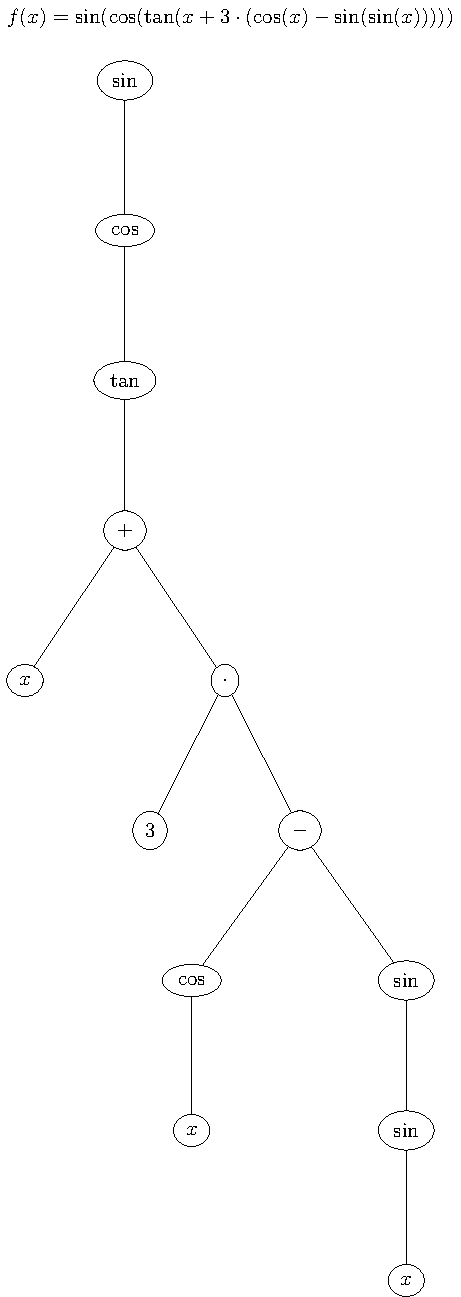
\includegraphics[width=0.52\linewidth]{nasty_edward_equation.pdf}
    \caption{Expression tree for equation \ref{eq:nasty_edward_equation}}
    \label{fig:nasty_edward_equation}
\end{figure}


\noindent Recall the 8 functions from part 1 that you know the derivative to:
\begin{multicols}{2}
  \begin{enumerate}
    \item $x^{c}$  \item $e^{x}$ \item $\ln(x)$ \item $\sin(x)$
    \item $\cos(x)$ \item $\tan(x)$ \item $\csc(x)$ \item $\sec(x)$
  \end{enumerate}
\end{multicols}

\noindent \textbf{Question 3}
The following functions are composed of the previous building block functions. For each, identify each piece of the nested function.

\begin{multicols}{2}
\noindent (a)
\begin{align*}
    f(g(h(k(x))))&=-e^{\left(\sin\left(x^{3}\right)\right)^{5}}\\
    g(h(k(x)))&=\left(\sin\left(x^{3}\right)\right)^{5}\\
    h(k(x))&=\sin\left(x^{3}\right)\\
    k(x)&=x^{3}
\end{align*}
\noindent (c)
\begin{align*}
    f(g(h(k(x))))&=\left[\csc\left(e^{5\sqrt{x}}\right)\right]^{3}\\
    g(h(k(x)))&=\\
    h(k(x))&=\\
    k(x)&=
\end{align*}

\columnbreak

\noindent (b)
\begin{align*}
    f(g(h(k(x))))&=\tan\left(\sin\left(\ln\left(x^{2}\right)\right)\right)\\
    g(h(k(x)))&=\\
    h(k(x))&=\\
    k(x)&=
\end{align*}
\noindent (d)
\begin{align*}
    f(g(h(k(x))))&=\text{another function}\\
    g(h(k(x)))&=\\
    h(k(x))&=\\
    k(x)&=
\end{align*}
\end{multicols}



\pagebreak

\section{Applying the chain rule}
\noindent A derivative is (essentially) division. $\frac{dy}{dx}$ is the change in $y$ \underline{\textbf{divided by}} the corresponding change in $x$. To this end, if we wanted to take the derivative of a nested function $f(g(h(x)))$, then the following steps can be taken:
\begin{align}
    &\frac{d}{dx}f(g(h(x))) \\
    =& \frac{d}{dx}f(g(h(x)))\left(\frac{dg(h(x))}{dg(h(x))}\right)\left(\frac{dh(x)}{dh(x)}\right) \\
    =& \frac{d}{dx}f(g(h(x)))\cdot\frac{d}{dg(h(x))}g(h(x))\cdot \frac{d}{dh(x)}h(x) \\
    =& \frac{d}{dg(h(x))}f(g(h(x)))\cdot\frac{d}{dh(x)}g(h(x))\cdot \frac{d}{dx}h(x)
\end{align}
which is the definition of the chain rule.
\\
Using this outline, we can construct the derivative of our first nested function:
\begin{align*}
&\left[\frac{d}{d(\sin(x^{3}))^{5}}-e^{(\sin(x^{3}))^{5}}\right] \cdot \left[\frac{d}{d\sin(x^{3})}(\sin(x^{3}))^{5}\right] \cdot \left[\frac{d}{dx^{3}}\sin(x^{3})\right] \cdot \left[\frac{d}{dx}x^{3}\right] \\
=&\left[-e^{(\sin(x^{3}))^{5}}\right] \cdot \left[5(\sin(x^{3}))^{4}\right] \cdot \left[\cos(x^{3})\right] \cdot \left[3x^{2}\right]
\end{align*}

\vspace{.5cm}

\noindent \textbf{Question 4}
Now do the same with nested functions (b), (c), and (d) from Question 3:

\pagebreak

\section{Exquisite Corpse Function}
\noindent With your group, choose 5 functions from the 8 building block functions in part-2. Next, add them, multiply them, or compose them to create one monster function. E.g. $f\Big(g\big(h(x)\big)\cdot k\big(m(x)\big)\Big)$, or $f\Big(g\big(h(k(x)+m(x))\big)\Big)$. Write your function below:\\
\vspace{3cm}

\noindent \textbf{Question 5} Exchange/rotate your function with the other groups. Solve their monster function below:

\pagebreak

\subsection{Sample Questions}
\begin{enumerate}
    \item $$y = \ln(f(x))$$
    \item $$y = f(cos(x))$$
    \item $$y = (f(x))^{3}$$
    \item $$y = e^{f(x)}$$
    \item $$y = 5\sin(f(x))$$
    \item $$y = \sec(f(x)g(x))$$
    \item $$y = f(g(h(x)))$$
\end{enumerate}
\end{document}
